\documentclass{report}

\usepackage{amsmath,amsfonts,amsthm,amssymb}
\usepackage{setspace}
\usepackage{Tabbing}
\usepackage{fancyhdr}
\usepackage{lastpage}
\usepackage{extramarks}
\usepackage{chngpage}
\usepackage{soul,color}
\usepackage{graphicx,float,wrapfig}
\usepackage{graphicx}
\usepackage{listings}
\usepackage{color}
\usepackage{multirow}

% Some configurations
\graphicspath{ {images/} }
\lstset {language=C++}

% In case you need to adjust margins:
\topmargin=-0.45in      %
\evensidemargin=0in     %
\oddsidemargin=0in      %
\textwidth=6.5in        %
\textheight=9.0in       %
\headsep=0.25in         %

% Homework Specific Information
\newcommand{\tpTitle}{TP\ 1 - Scheduling}
\newcommand{\materia}{SO}

% Setup the header and footer
\pagestyle{fancy}                                    %  
\fancyhead{}                                         % Remove all header contents
\renewcommand{\headrulewidth}{0pt}                   % Remove header line
\lfoot{\lastxmark}                                   %
\cfoot{}                                             %
\rfoot{Page\ \thepage\ of\ \pageref{LastPage}}       %
\renewcommand\footrulewidth{0.4pt}                   %

%%%%%%%%%%%%%%%%%%%%%%%%%%%%%%%%%%%%%%%%%%%%%%%%%%%%%%%%%%%%%
% Some tools
\newcommand{\enterProblemHeader}[1]{\nobreak\extramarks{#1}{#1 continued on next page\ldots}\nobreak%
                                    \nobreak\extramarks{#1 (continued)}{#1 continued on next page\ldots}\nobreak}%
\newcommand{\exitProblemHeader}[1]{\nobreak\extramarks{#1 (continued)}{#1 continued on next page\ldots}\nobreak%
                                   \nobreak\extramarks{#1}{}\nobreak}%

\newlength{\labelLength}
\newcommand{\labelAnswer}[2]
  {\settowidth{\labelLength}{#1}%
   \addtolength{\labelLength}{0.25in}%
   \changetext{}{-\labelLength}{}{}{}%
   \noindent\fbox{\begin{minipage}[c]{\columnwidth}#2\end{minipage}}%
   \marginpar{\fbox{#1}}%

   % We put the blank space above in order to make sure this
   % \marginpar gets correctly placed.
   \changetext{}{+\labelLength}{}{}{}}%

\setcounter{secnumdepth}{0}
\newcommand{\homeworkProblemName}{}%
\newcounter{homeworkProblemCounter}%
\newenvironment{homeworkProblem}[1][Problem \arabic{homeworkProblemCounter}]%
  {\stepcounter{homeworkProblemCounter}%
   \renewcommand{\homeworkProblemName}{#1}%
   \section{\homeworkProblemName}%
   \enterProblemHeader{\homeworkProblemName}}%
  {\exitProblemHeader{\homeworkProblemName}}%

\newcommand{\problemAnswer}[1]
  {\noindent\fbox{\begin{minipage}[c]{\columnwidth}#1\end{minipage}}}%

\newcommand{\problemLAnswer}[1]
  {\labelAnswer{\homeworkProblemName}{#1}}

\newcommand{\homeworkSectionName}{}%
\newlength{\homeworkSectionLabelLength}{}%
\newenvironment{homeworkSection}[1]%
  {% We put this space here to make sure we're not connected to the above.
   % Otherwise the changetext can do funny things to the other margin

   \renewcommand{\homeworkSectionName}{#1}%
   \settowidth{\homeworkSectionLabelLength}{\homeworkSectionName}%
   \addtolength{\homeworkSectionLabelLength}{0.25in}%
   \changetext{}{-\homeworkSectionLabelLength}{}{}{}%
   \subsection{\homeworkSectionName}%
   \enterProblemHeader{\homeworkProblemName\ [\homeworkSectionName]}}%
  {\enterProblemHeader{\homeworkProblemName}%

   % We put the blank space above in order to make sure this margin
   % change doesn't happen too soon (otherwise \sectionAnswer's can
   % get ugly about their \marginpar placement.
   \changetext{}{+\homeworkSectionLabelLength}{}{}{}}%

\newcommand{\sectionAnswer}[1]
  {% We put this space here to make sure we're disconnected from the previous
   % passage

   \noindent\fbox{\begin{minipage}[c]{\columnwidth}#1\end{minipage}}%
   \enterProblemHeader{\homeworkProblemName}\exitProblemHeader{\homeworkProblemName}%
   \marginpar{\fbox{\homeworkSectionName}}%

   % We put the blank space above in order to make sure this
   % \marginpar gets correctly placed.
   }%

%%%%%%%%%%%%%%%%%%%%%%%%%%%%%%%%%%%%%%%%%%%%%%%%%%%%%%%%%%%%%


%%%%%%%%%%%%%%%%%%%%%%%%%%%%%%%%%%%%%%%%%%%%%%%%%%%%%%%%%%%%%
% Make title
\title{\vspace{2in}\textmd{\textbf{\materia:\ \tpTitle}}}
\date{}
\author{
  Andreas Sturmer\\
  \texttt{COMPLETAR@xxxxx.com}
  \and
  Dan Zajdband\\
  \texttt{dan.zajdband@gmail.com}
  \and
  Javier Casal\\
  \texttt{javierjcasal@gmail.com}
}
%%%%%%%%%%%%%%%%%%%%%%%%%%%%%%%%%%%%%%%%%%%%%%%%%%%%%%%%%%%%%

\begin{document}
\begin{spacing}{1.3}
\maketitle
\newpage
% Uncomment the \setcounter line as well if you do NOT want subsections
%       listed in Contents
\tableofcontents
\newpage

\clearpage
\begin{homeworkProblem}[Ejercicio 1]
    En este primer ejercicio se nos pide programar una tarea interactiva que realice  \textit{n} llamadas bloqueantes de una duraci\'on al azar comprendida entre dos de los par\'ametros que la tarea recibe (el tercer par\'ametro es \textit{n}, es decir, la mencionada cantidad de llamadas bloqueantes).\\

\textbf{Implementaci\'on} \\
        Para ello empezamos por registrar la tarea en la funci\'on provista \textit{tasks\_init} seg\'un se indica. Luego implementamos la funci\'on reci\'en registrada vali\'endonos de la funci\'on \textit{uso\_IO} que resulta en una llamada bloqueante de \textit{t} ciclos de reloj en completar (donde \textit{t} es el \'unico par\'ametro que \textit{uso\_IO} recibe. Falta \'unicamente mencionar que, para definir un tiempo al azar que est\'e comprendido entre los valores solicitados, realizamos una suma que adicione el m\'inimo necesario a un valor aleatroio comprendido entre la diferencia entre el m\'inimo (\textit{bmin}) y el m\'aximo (\textit{bmax}) recibidos:
            \begin{center}
            bmin + (rand() \% ((bmax + 1) - bmin))
            \end{center} 

\textbf{Gr\'afico de un lote de tareas} \\
        El gr\'afico a continuaci\'on (\textit{Figure 1}) corresponde a un lote de 1 tarea que realiza 4 llamadas bloqueantes de entre 2 y 7 tiempos de duraci\'on: \\
        \begin{figure}[h]
            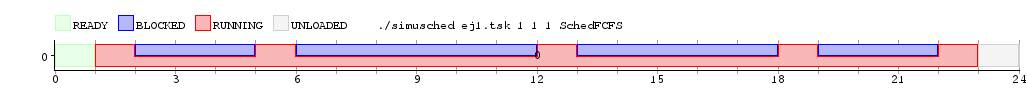
\includegraphics[width=1\textwidth]{ej1}
            \caption{}
        \end{figure} \\
No son muchas las cosas a revisar, entre ellas: \\
- Las llamadas bloqueantes son, en efecto, 4 \\
- Las llamadas bloqueantes en ning\'un caso duran menos de 2 tiempos \\
- Las llamadas bloqueantes en ning\'un caso se exceden de 7 tiempos de duraci\'on

\end{homeworkProblem}

\clearpage
\begin{homeworkProblem}[Ejercicio 2]
    En este segundo ejercicio estamos a cargo de Rolando, su complejo algoritmo, y sus distracciones al momento de sentarse a la computadora. \\
    Nuestro primer encargo es escribir un lote de tareas que simule la situaci\'on de Rolando descripta en el enunciado. Este lote incluye entonces una primer corrida de 100 ciclos de CPU en ning\'un caso bloqueantes buscando simular los 100 ciclos de corrida del algoritmo complejo de Rolando. Nos valemos para ello de la funci\'on provista \textit{TaskCPU}. Lo siguiente ser\'an 2 tareas con llamadas bloqueantes de una duraci\'on variable dentro de un rango; en otras palabras, 2 tareas que realizan exactamente aquello que se nos pidi\'o en el primer ejecicio del trabajo pr\'actico. Usamos entonces la tarea \textit{TaskConsola} con los par\'ametros correspondientes para simular las tareas de ocio de Rolando. \\
    
    \textbf{Gr\'aficos utilizando 1 y 2 n\'ucleos} \\
    Los gr\'aficos a continuaci\'on (\textit{Figure 2}) corresponden a la ejecuci\'on de la simulaci\'on utilizando el algoritmo FCFS para 1 core (Figure 2) y para 2 cores (Figure 3). En ambos casos el costo de cambio de contexto es de 4 ciclos.
    
    \begin{figure}[h]
        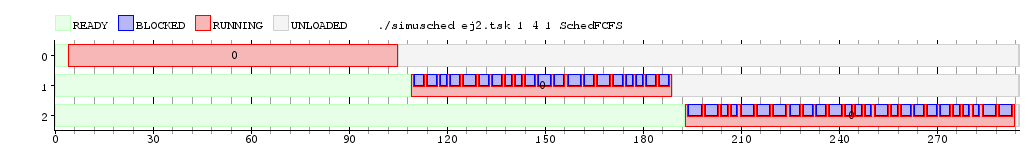
\includegraphics[width=1\textwidth]{ej2-1core}
        \caption{}
    \end{figure}
    
    \begin{figure}[h]
        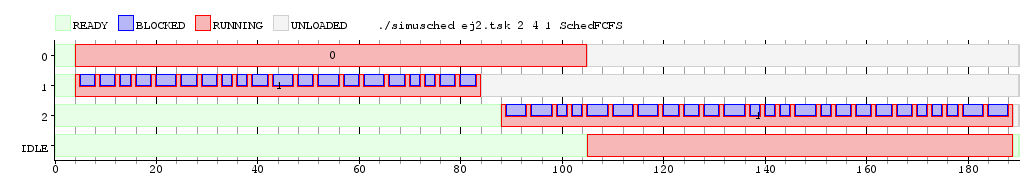
\includegraphics[width=1\textwidth]{ej2-2core}
        \caption{}
    \end{figure}

    \textbf{Latencia} \\
    La siguiente asignatura es el c\'alculo de la latencia de cada una de las tareas en cada uno de los dos casos:
\begin{table}[h]
  \begin{center}
\begin{tabular}{c|c|c|c}
        & Tarea 1 & Tarea 2 & Tarea 3 \\
\hline
1 core  & 4       & 109     & 193     \\
\hline
2 cores & 4       & 4       & 88     
\end{tabular}
  \end{center}
\end{table}
    
    
\end{homeworkProblem}

\clearpage
\begin{homeworkProblem}[Ejercicio 3]
    Work in progress...
\end{homeworkProblem}

\clearpage
\begin{homeworkProblem}[Ejercicio 4]
    Work in progress...
\end{homeworkProblem}

\clearpage
\begin{homeworkProblem}[Ejercicio 5]
    Work in progress...
\end{homeworkProblem}

\clearpage
\begin{homeworkProblem}[Ejercicio 6]
    Work in progress...
\end{homeworkProblem}

\clearpage
\begin{homeworkProblem}[Ejercicio 7]
    Work in progress...
\end{homeworkProblem}

\clearpage
\begin{homeworkProblem}[Ejercicio 8]
    Work in progress...
\end{homeworkProblem}


\end{spacing}
\end{document}

%%%%%%%%%%%%%%%%%%%%%%%%%%%%%%%%%%%%%%%%%%%%%%%%%%%%%%%%%%%%%

%----------------------------------------------------------------------%
% The following is copyright and licensing information for
% redistribution of this LaTeX source code; it also includes a liability
% statement. If this source code is not being redistributed to others,
% it may be omitted. It has no effect on the function of the above code.
%----------------------------------------------------------------------%
% Copyright (c) 2007, 2008, 2009, 2010, 2011 by Theodore P. Pavlic
%
% Unless otherwise expressly stated, this work is licensed under the
% Creative Commons Attribution-Noncommercial 3.0 United States License. To
% view a copy of this license, visit
% http://creativecommons.org/licenses/by-nc/3.0/us/ or send a letter to
% Creative Commons, 171 Second Street, Suite 300, San Francisco,
% California, 94105, USA.
%
% THE SOFTWARE IS PROVIDED "AS IS", WITHOUT WARRANTY OF ANY KIND, EXPRESS
% OR IMPLIED, INCLUDING BUT NOT LIMITED TO THE WARRANTIES OF
% MERCHANTABILITY, FITNESS FOR A PARTICULAR PURPOSE AND NONINFRINGEMENT.
% IN NO EVENT SHALL THE AUTHORS OR COPYRIGHT HOLDERS BE LIABLE FOR ANY
% CLAIM, DAMAGES OR OTHER LIABILITY, WHETHER IN AN ACTION OF CONTRACT,
% TORT OR OTHERWISE, ARISING FROM, OUT OF OR IN CONNECTION WITH THE
% SOFTWARE OR THE USE OR OTHER DEALINGS IN THE SOFTWARE.
%----------------------------------------------------------------------%
